\documentclass[10pt,a4paper,hidelinks]{article}
\usepackage[hyphens]{url}
\usepackage[latin2]{inputenc}
\usepackage{graphicx}
\usepackage{amsmath}
\usepackage{amsfonts}
\usepackage{amssymb}
\usepackage{makeidx}
\usepackage{float}
\usepackage{hyperref}
\usepackage{geometry}

\author{Marko Mihelin}
\title{SensorLab VESNA open source development environment setup guide for Windows based development}

\makeindex
\begin{document}

% title page
\begin{titlepage}
    \begin{center}
    \textbf{
        \raisebox{-0.4\height}{
            
\includegraphics[width=1cm]{./install-guide-win-images/jsi-logo.png}
        }
        \Large ``Jo�ef Stefan'' Institute \\[2mm]
        \raisebox{-0.4\height}{
            
\includegraphics[width=1cm]{./install-guide-win-images/comms-logo.png}
        }
        Department of Communication Systems\\[2mm]
        
\includegraphics[height=1cm]{./install-guide-win-images/sensorlab-logo.png}
        }

    \vfill

    \textbf{\huge SensorLab VESNA open source development environment setup guide
        for Windows based development}\\[1.5cm]


    \textbf{ \Large
    version 0.10}\\[1cm]

    \textnormal{\Large
    by Marko Mihelin}\\[1cm]

    \vfill

    \textnormal{\large
    \today\\[1cm]
    }
    \end{center}
\end{titlepage}

\newpage

\section{Introduction}
The setup and usage of the open source development environment for the VESNA platform is described in this document.  This manual is for Windows based development and has been successfully tested on Windows 7 and 8, 32bit and 64bit versions.

\subsection{Overview of the installation process}

\begin{enumerate}
\item Install Cygwin
\item Install CodeBench tool-chain
\item Install OpenOCD
\item Install ST Flash Loader Demonstrator (Optional)
\item Install Eclipse
\item Install Eclipse plug-ins (tool-chain support, debugging support, ...)
\item Connect the debugger interface and install the drivers
\item Download VESNA repository, build and debug
\end{enumerate}
 
\newpage

\tableofcontents
\newpage

\listoffigures
\newpage

\subsection*{List of Abbreviations}
	\begin{tabular}{ l l }
	IDE		& Integrated Development Environment \\
	SNC		& Sensor Node Core module \\
	MRAM	& Magnetoresistive random-access memory \\
	\end{tabular}
\newpage
 
\section{Install Cygwin}

Cygwin is a  Linux-like environment for Windows. It is needed because the build process of the projects require some Linux specific commands that Cygwin provides. You can download it from \url{http://cygwin.com/}. The version at the time of writing was 1.7.30. You can install it with default options. Make sure you add the \textit{"C:\textbackslash install\textbackslash dir\textbackslash cygwin\textbackslash bin"} to your system PATH. You do this by going to Control Panel and clicking on System. Got to \textit{Advanced system settings $\rightarrow$ Environment Variables}.

	\begin{figure}[H]
	\centering
	    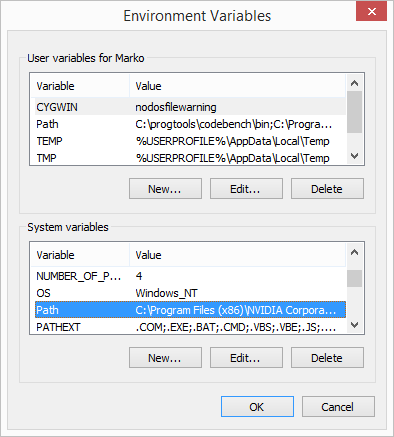
\includegraphics[scale=0.7]{./install-guide-win-images/environment-variables.png}
	    \caption{Selecting the PATH environment variable}
	    \label{fig:environment-variables}
	\end{figure}
    
Now find the variable \textit{PATH} in the \textit{System Variables} window, select it and click edit (\autoref{fig:environment-variables}).

	\begin{figure}[H]
	\centering
	    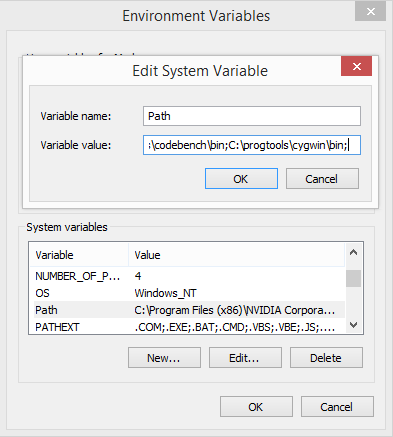
\includegraphics[scale=0.7]{./install-guide-win-images/environment-variables-path.png}
	    \caption{Add new path to PATH variable}
	    \label{fig:environment-variables-path}
	\end{figure}

At the end of the string of paths in \textit{"Variable value"} field add a semicolon (;) and the path to Cygwin install directory like in \autoref{fig:environment-variables-path}. Make sure not to delete any preexisting paths. Click \textit{OK}.

\newpage

\section{Install Sourcery CodeBench tool-chain}

The tool-chain contains the compiler linker and debugger for ARMv7M software development. The tool-chain can be download from \url{http://www.mentor.com/embedded-software/sourcery-tools/sourcery-codebench/editions/lite-edition/arm-eabi}. You have to provide your name and e-mail. A download link will be sent to you via e-mail. Select the \textit{"Sourcery CodeBench Lite 2013.11-24"} release. Newer releases may also work but were not tested at the time of writing.
Start the installation.

	\begin{figure}[H]
	\centering
	    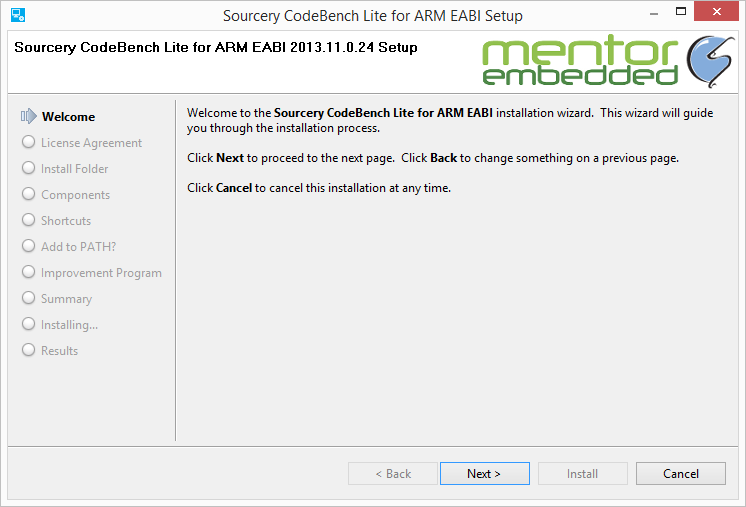
\includegraphics[width=0.9\textwidth]{./install-guide-win-images/codebench-install.png}
	    \caption{Tool-chain installation welcome window}
	    \label{fig:codebench-install}
	\end{figure}

Chose an install path with no spaces (spaces can cause problems with Eclipse, and the debugger) (\autoref{fig:codebench-install}).

	\begin{figure}[H]
	\centering
	    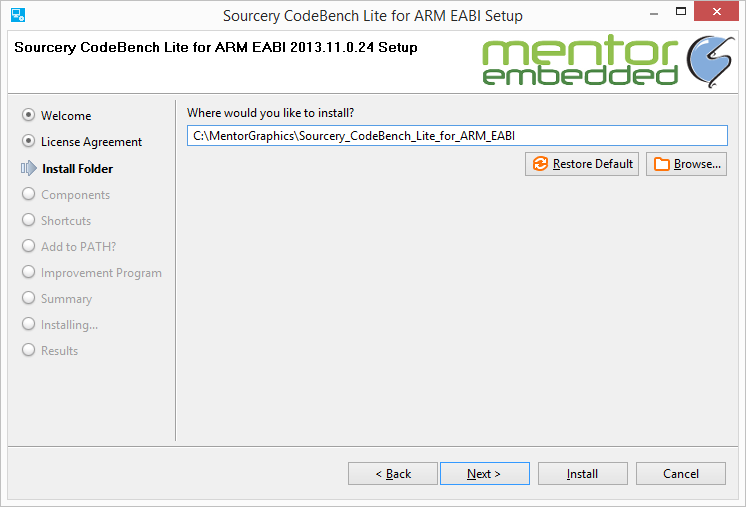
\includegraphics[width=0.9\textwidth]{./install-guide-win-images/codebench-install-location.png}
	    \caption{Modify PATH for all users}
	    \label{fig:codebench-install-location}
	\end{figure}

Select \textit{"Modify PATH for current users"} (\autoref{fig:codebench-install-location}). Finish the installation. Make sure that path to the tool-chain was added to \textit{System PATH}.

\newpage

\section{Install OpenOCD}

OpenOCD is the interface between the hardware JTAG and the debugger, the current stable version is 0.8.0. It can be build form source or a precompiled binary can be downloaded from  \url{http://www.freddiechopin.info/en/download/category/4-openocd}. Select the 0.8.0 version. Unzip the folder where you want to place OpenOCD. Make sure that the installation path does not contain any spaces or non-US characters. Then go to the unzip folder and rename it form \textit{OpenOCD-0.8.0} to \textit{OpenOCD}. Go to sub-folder \textit{bin} or \textit{bin-x64} (depending on your system, 32bit or 64bit Windows) and rename \textit{openocd*.exe} to \textit{openocd.exe}. Add the \textit{bin} or \textit{bin-x64} (again, depending on your system) folder to your \textit{System PATH}.

\section{Install ST Flash Loader Demonstrator (Optional)}

The Flash Loader can upload software to target microcontroller using only a com port. It can upload binary .bin or .s19 images. This is useful for programing SNC when JTAG can not be used, for instance when using the on-board MRAM. The Flash loader can be downloaded from ST \href{http://www.st.com/web/en/catalog/tools/PF257525#}{ST Flash Loader Demonstartor}. To initialize the on-board bootloader you must push and hold the button on the SNC for more then 5 seconds. Then use the Flash loader to connect and upload the software.

\section{Install Eclipse IDE}

Before installing Eclipse you must have the latest 32bit \textit{Java Run-time Environment} installed. You can find it at \url{https://www.java.com/en/}.

\subsection{Install Eclipse}

Eclipse can be downloaded from \url{http://www.eclipse.org/downloads/}. The newest release at the time of writing was Kepler (4.3). Newer releases may also work but are not yet tested. Select the \textit{"Eclipse IDE for C/C++ Developers"} 32bit version and download it. Eclipse does not need installation, just unzip in a desired location and run it. 
Start Eclipse now. You are prompted for workspace location (\autoref{fig:eclipse-workspace-select}), this is were the settings are stored. You can select the default location. Make sure the path name does not contain any non-US characters and spaces.

	\begin{figure}[H]
	\centering
	    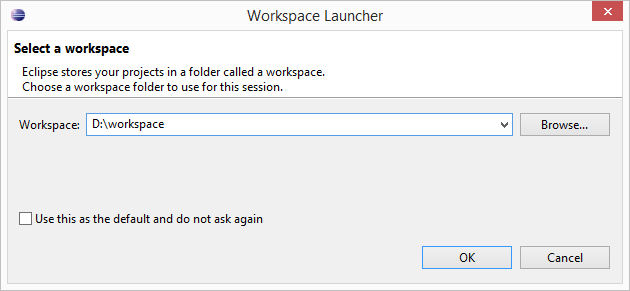
\includegraphics[scale=0.7]{./install-guide-win-images/eclipse-workspace-select.png}
	    \caption{Eclipse workspace prompt}
	    \label{fig:eclipse-workspace-select}
	\end{figure}

You are presented with a welcome window (\autoref{fig:eclipse-welcome}).
 
	\begin{figure}[H]
	\centering
	    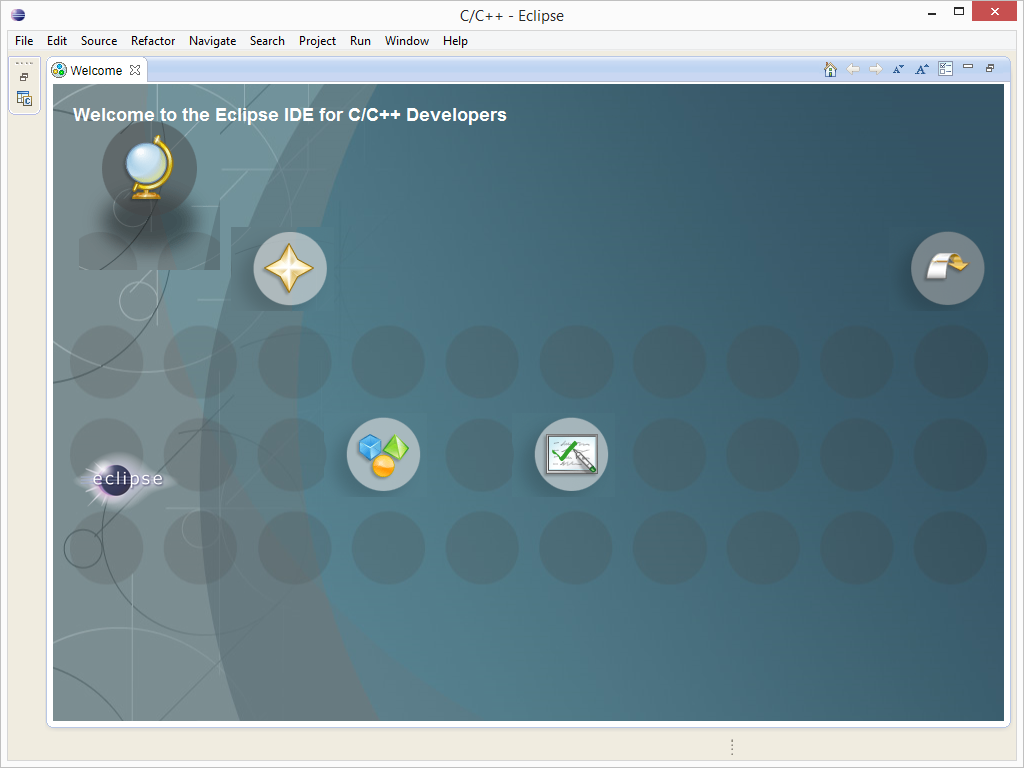
\includegraphics[width=0.9\textwidth]{./install-guide-win-images/eclipse-welcom.png}
	    \caption{Eclipse welcome window}
	    \label{fig:eclipse-welcome}
	\end{figure}
	
Now you have to install some plug-ins.

\newpage

\subsection{Install the GNU ARM Development support}

Go to \textit{Help $\rightarrow$ Install new software...} window and paste this URL \textit{"http://gnuarmeclipse.sourceforge.net/updates"} to the \textit{"Work with"}  line (\autoref{fig:eclipse-plugin-install-gnuarm}). Install the plug-in.

	\begin{figure}[H]
	\centering
	    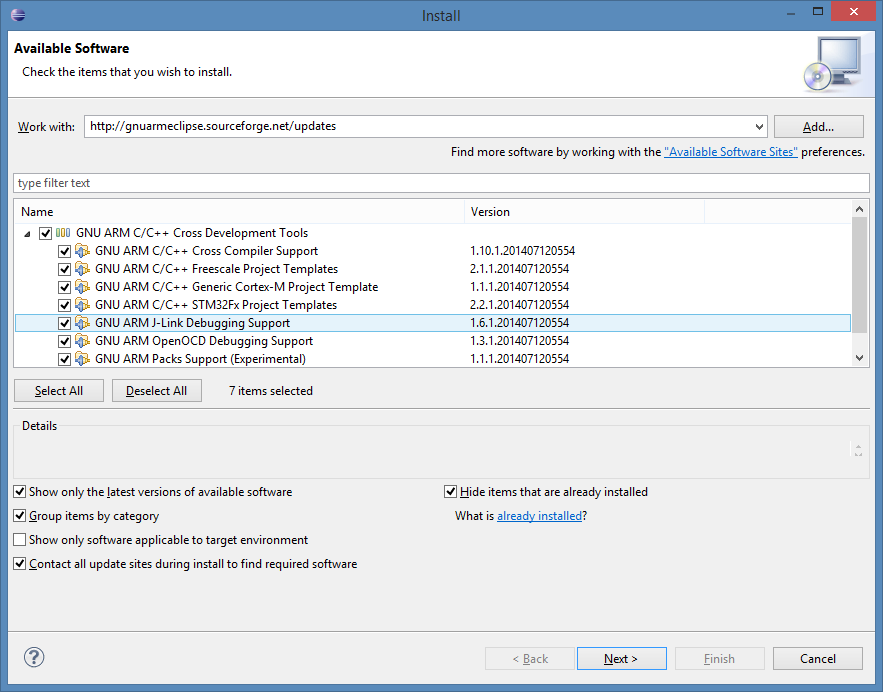
\includegraphics[width=0.9\textwidth]{./install-guide-win-images/eclipse-plugin-install-gnuarm.png}
	    \caption{Install GNU ARM development support}
	    \label{fig:eclipse-plugin-install-gnuarm}
	\end{figure}

This plug-in adds automatic makefile creation capabilities and tool-chain preconfiguration to Eclipse. It supports various opensource tool-chains.

\newpage

\subsection{Install the Zylin CDT plug-in}

To install the Zylin CDT plug-in go again to the \textit{"Install new software"} window and paste this URL \textit{"http://opensource.zylin.com/zylincdt"} select the plug-in and install it (\autoref{fig:eclipse-plugin-install-zylin}).

	\begin{figure}[H]
	\centering
	    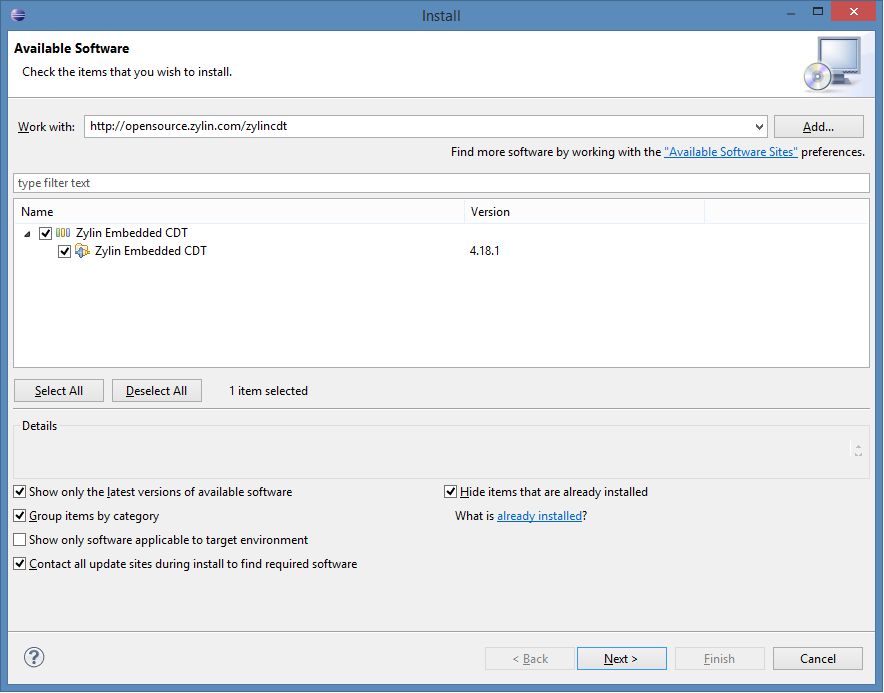
\includegraphics[width=0.9\textwidth]{./install-guide-win-images/eclipse-plugin-install-zylin.png}
	    \caption{Install the Zylin Embedded CDT}
	    \label{fig:eclipse-plugin-install-zylin}
	\end{figure}
	
The Zylin CDT plug-in enables Eclipse to communicate with GDB debugger.

\newpage

\subsection{Install the EmbSys peripheral register view plug-in}

To install the EmbSys peripheral register view plug-in go to the  \textit{"Install new software"} window and paste this URL \textit{"http://embsysregview.sourceforge.net/update"} select the plug-in and install it (\autoref{fig:eclipse-plugin-install-embsys}).

	\begin{figure}[H]
	\centering
	    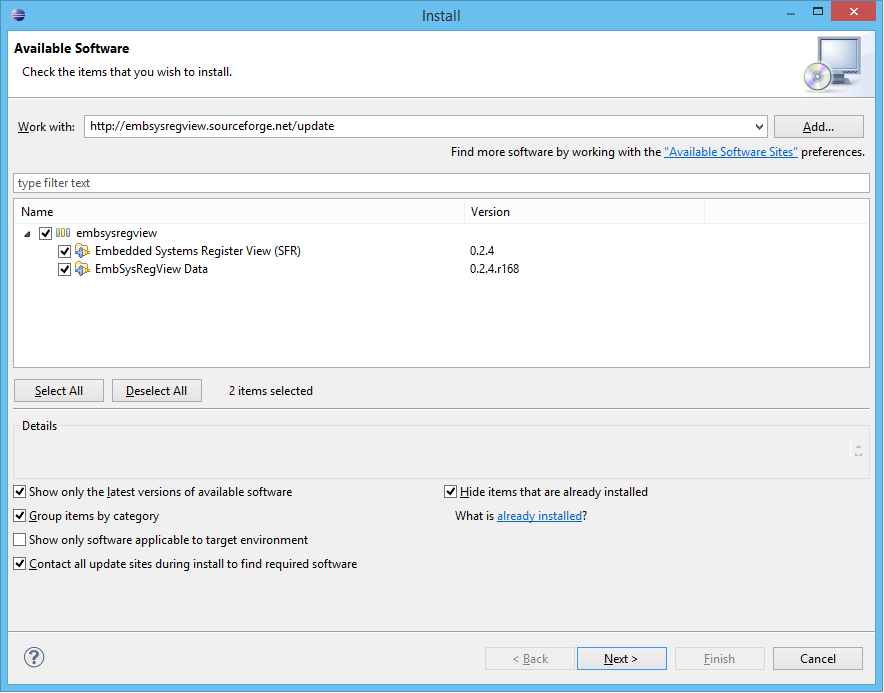
\includegraphics[width=0.9\textwidth]{./install-guide-win-images/eclipse-plugin-install-embsys.png}
	    \caption{EmbSys Register View plug-in installation}
	    \label{fig:eclipse-plugin-install-embsys}
	\end{figure}

After installation go to \textit{Window $\rightarrow$ Preferences $\rightarrow$ C/C++ $\rightarrow$ Debug $\rightarrow$ EmbSys} Register view to setup the plug-in. For \textit{Architecture} select \textit{cortex m3}, for \textit{Vendor} select \textit{STMicro} and for \textit{Chip} select \textit{STM32F10x\_HD\_VL} click \textit{OK} (\autoref{fig:eclipse-plugin-config-embsys}). To add the plug-in into a view go to \textit{Window $\rightarrow$ Show View $\rightarrow$ Other... $\rightarrow$ Debug} and select \textit{EmbSys Register}. Now you can view and change the peripheral registers of the microcontroller when debugging (\autoref{fig:eclipse-plugin-view-embsys}).

	\begin{figure}[H]
	\centering
	    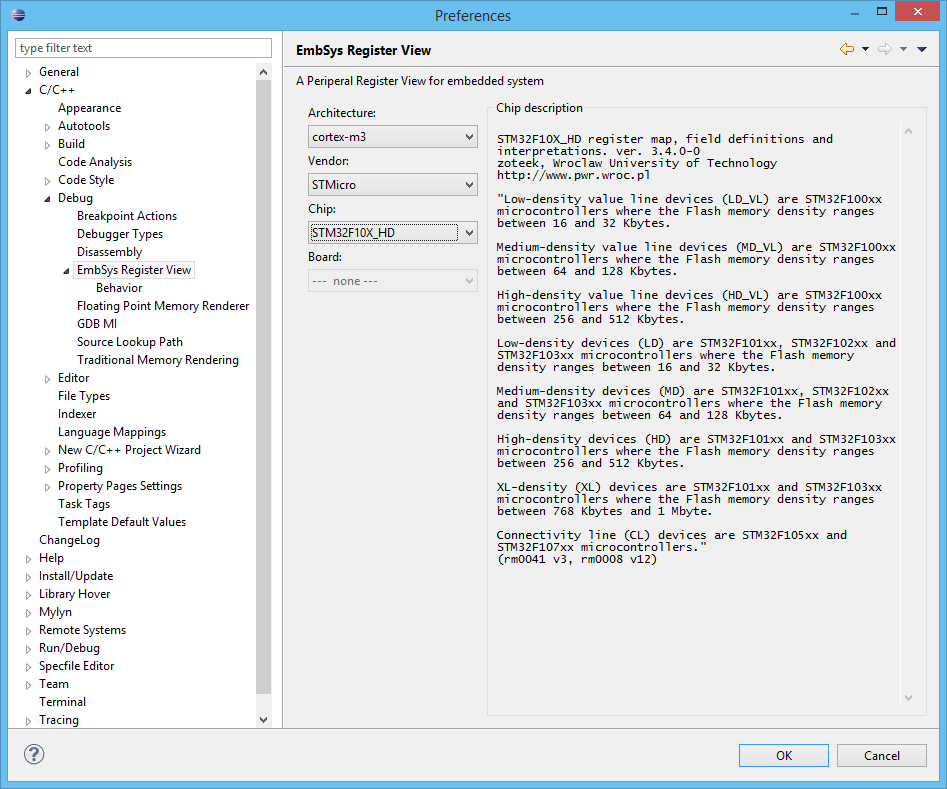
\includegraphics[width=0.9\textwidth]{./install-guide-win-images/eclipse-plugin-config-embsys.png}
	    \caption{EmbSys Register View setup}
	    \label{fig:eclipse-plugin-config-embsys}
	\end{figure}

	\begin{figure}[H]
	\centering
	    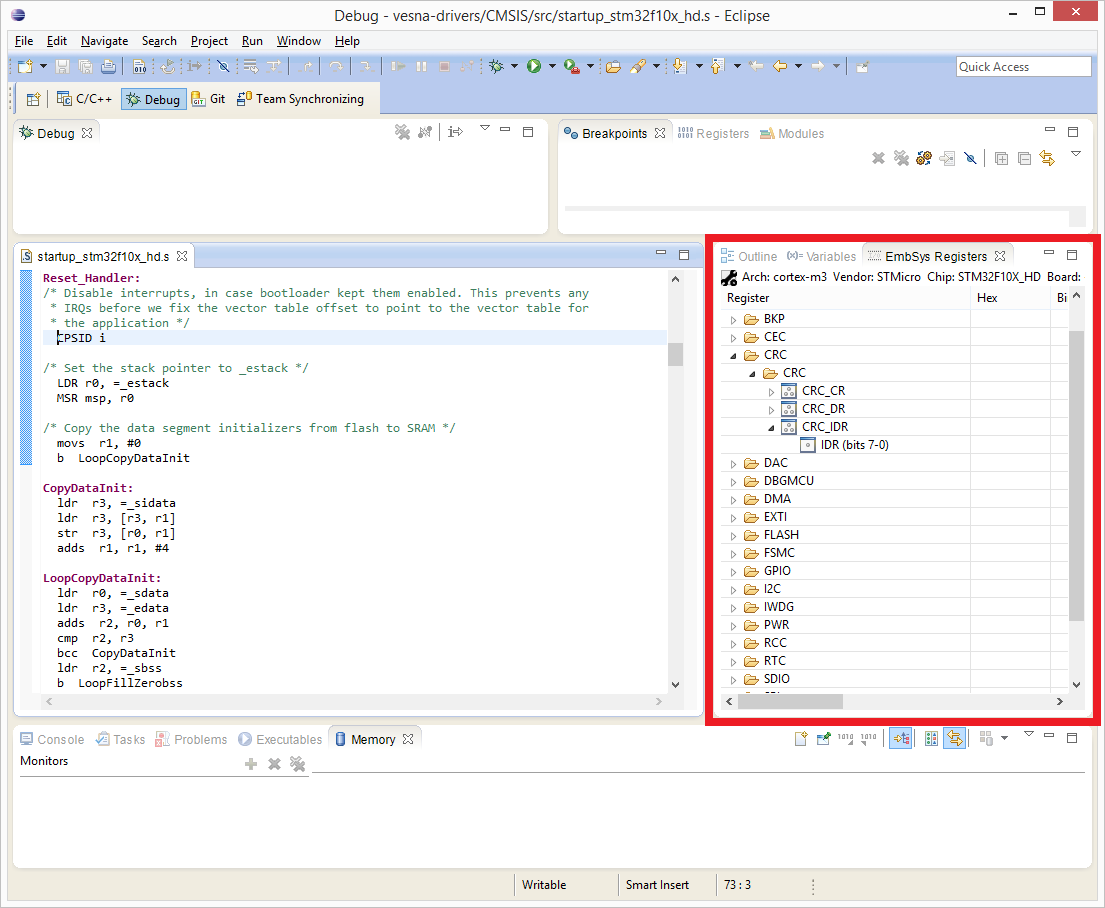
\includegraphics[width=0.9\textwidth]{./install-guide-win-images/eclipse-plugin-view-embsys.png}
	    \caption{EmbSys Register view (red square)}
	    \label{fig:eclipse-plugin-view-embsys}
	\end{figure}

\newpage
	
\subsection{Configure Eclipse Git client}

A Git client is already included in the base installation of Eclipse, you just need to configure it. Open \textit{Preferences} and navigate to \textit{Team $\rightarrow$ Git $\rightarrow$ Configuration} and add two new keys, email and name (\autoref{fig:eclipse-git-config}). You can use your Github credentials.

	\begin{figure}[H]
	\centering
	    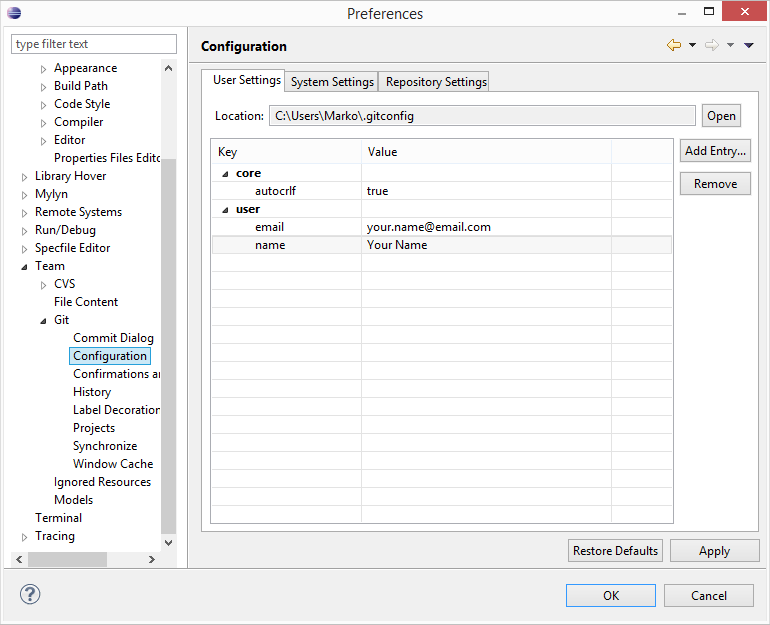
\includegraphics[width=0.9\textwidth]{./install-guide-win-images/eclipse-git-config.png}
	    \caption{Eclipse Git client configuration}
	    \label{fig:eclipse-git-config}
	\end{figure}

\newpage

\section{Connection of the debugger interface and installation of drivers}

In this section the installation of the ST-LINK/V2 hardware debugger interface is explained.

\begin{enumerate}
	\item First go to \url{http://www.st.com/web/catalog/tools/FM146/CL1984/SC724/SS1677/PF251168}, scroll down to the \textit{"Related Tools and Software"} section and download the appropriate USB driver for your Windows version (STSW-LINK003 for Win 7 or STSW-LINK006 for Win 8). Unzip the downloaded file.
	\item Now connect the debugger interface ST-LINK/V2 to the PC. Windows will not find the correct drivers for the debugger interface. Go to \textit{"Device Manager"} and install the drivers manually. 
	\item Go to \textit{"Other devices"} tab and look for an unknown device named \textit{"STM32 STLink"} (\autoref{fig:device-manager-stlink-no-driver}).
	
	\begin{figure}[H]
	\centering
		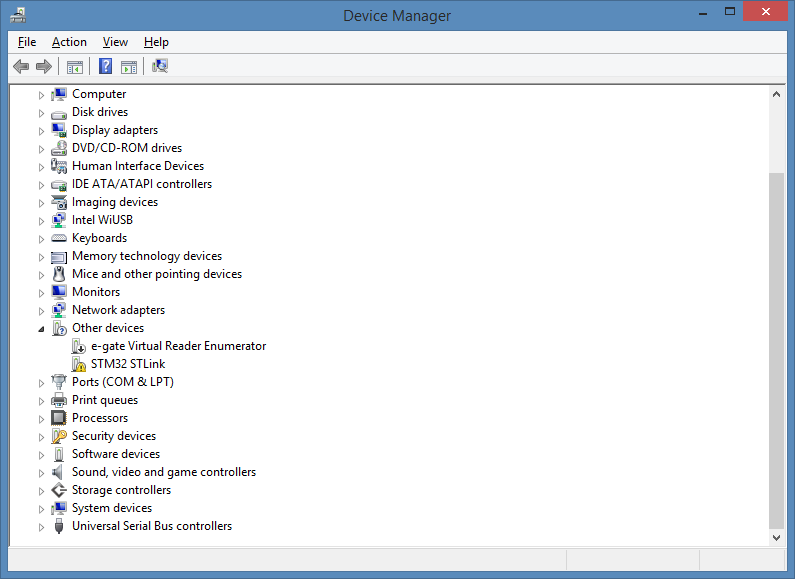
\includegraphics[width=0.9\textwidth]{./install-guide-win-images/device-manager-stlink-no-driver.png}
		\caption{Device Manager when STLink is connected for the first time}
		\label{fig:device-manager-stlink-no-driver}
	\end{figure}
	
	\item Right-click on it and click \textit{"Update Driver Software..."}
	\item In the new window click on \textit{"Browse my computer for driver software"} (\autoref{fig:device-manager-find-stlink-driver})
	
	\begin{figure}[H]
	\centering
		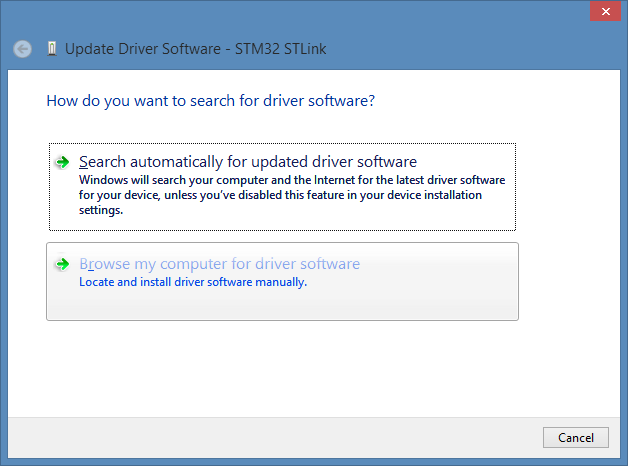
\includegraphics[scale=0.7]{./install-guide-win-images/device-manager-find-stlink-driver.png}
		\caption{Select method to find driver for STLink}
		\label{fig:device-manager-find-stlink-driver}
	\end{figure}	
	
	\item Browse to location where you've unzip the previously downloaded driver (\autoref{fig:device-manager-browse-stlink-driver}). Click next and the installation will start.

	\begin{figure}[H]	
	\centering
		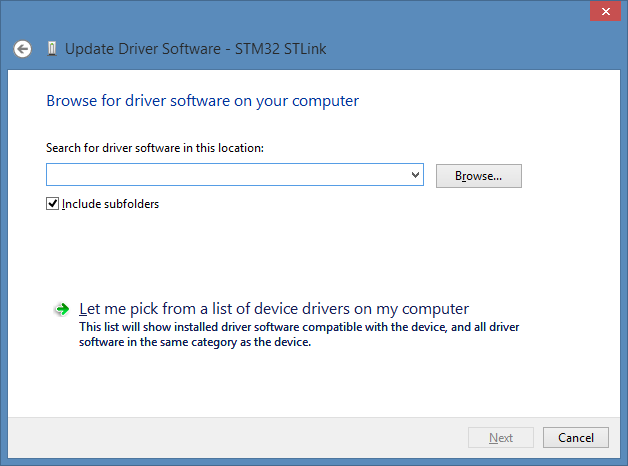
\includegraphics[scale=0.7]{./install-guide-win-images/device-manager-browse-stlink-driver.png}
		\caption{Browse to driver location}
		\label{fig:device-manager-browse-stlink-driver}
	\end{figure}		
	
	\item The driver is now installed (\autoref{fig:device-manager-stlink-driver-updated}).

	\begin{figure}[H]	
	\centering
		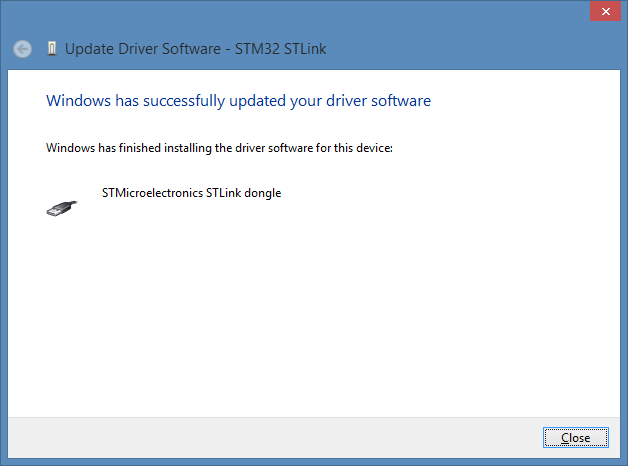
\includegraphics[scale=0.7]{./install-guide-win-images/device-manager-stlink-driver-updated.png}
		\caption{Driver installation complete}
		\label{fig:device-manager-stlink-driver-updated}
	\end{figure}
		
\end{enumerate}

\newpage

\section{Download VESNA repository, Build and Debug}

This chapter explains how to configure the Git plug-in, download the \textit{"vesna-drivers"} repository, compile the source code, upload the build binary file to SNC and start a debug session.
A Github (\url{https://github.com/}) account and access to the \textit{"vesna-drivers"} repository is a prerequisite for the completion of this section.
This guide does not cover the proper usage of Git or Github.

\subsection{Download  VESNA repository from Github}

In Eclipse open the \textit{"Git"} perspective. You can see that there are no available repositories. You can add the \textit{"vesna-drivers"} repository by clicking on \textit{"Clone a Git repository"} (\autoref{fig:eclipse-git-perspective}).

\begin{figure}[H]
\centering
	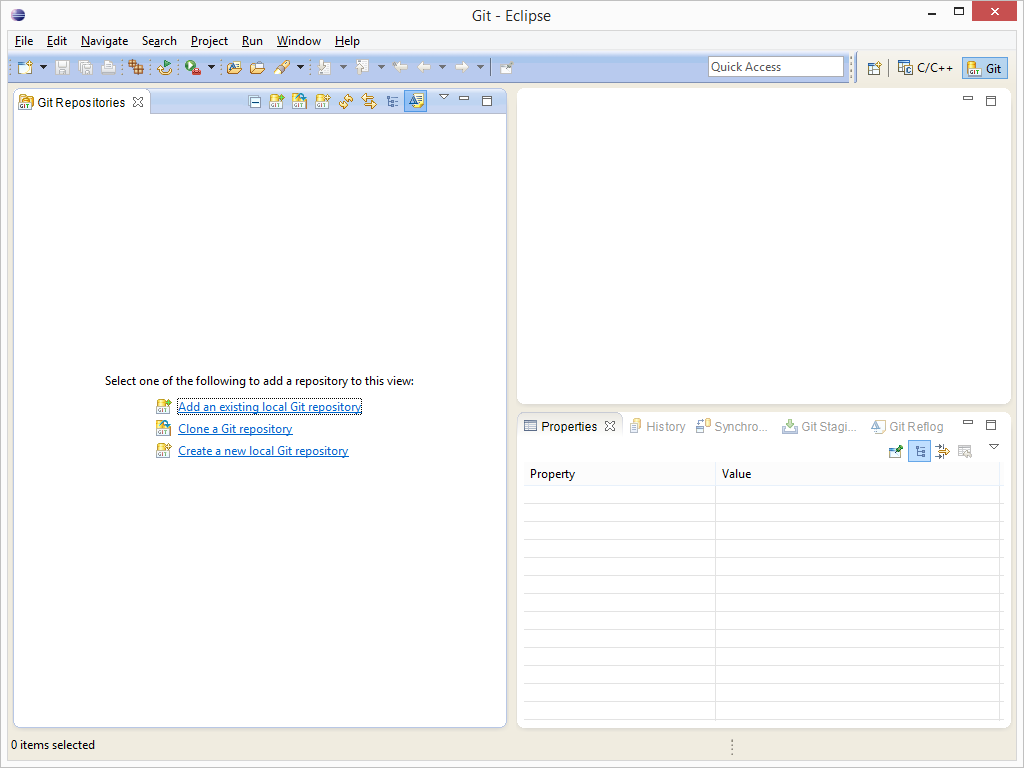
\includegraphics[width=0.9\linewidth]{./install-guide-win-images/eclipse-git-perspective.png}
	\caption{Git perspective in Eclipse}
	\label{fig:eclipse-git-perspective}
\end{figure}

Copy the repository URI: \textit{https://github.com/sensorlab/vesna-drivers.git} to the URI field (\autoref{fig:eclipse-git-clone-repo}). The other filed in Location frame should auto-complete. Fill in \textit{username} and \textit{password} of your Github account in the \textit{"Authentication"} frame. Click Next.

\begin{figure}[H]
\centering
	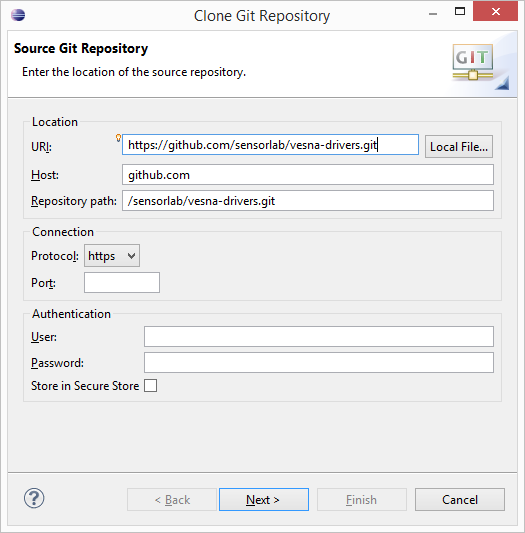
\includegraphics[scale=0.7]{./install-guide-win-images/eclipse-git-clone-repo.png}
	\caption{Git repository location and credentials}
	\label{fig:eclipse-git-clone-repo}
\end{figure}

Now you will be presented with a branch selection window. Select only the \textit{"master"} branch as it is the most current (\autoref{fig:eclipse-git-clone-repo-branch-selection}). Click Next.

\begin{figure}[H]
\centering
	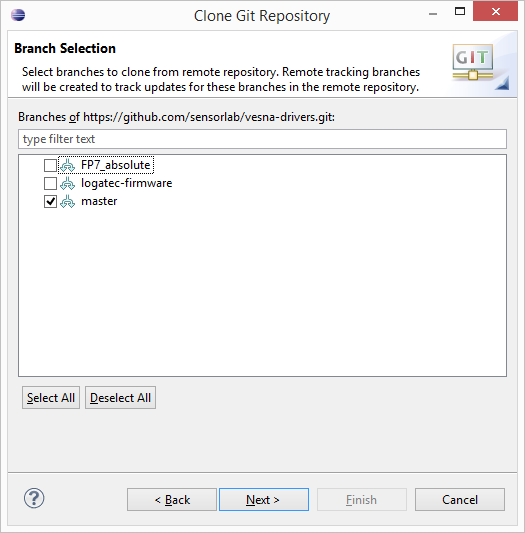
\includegraphics[scale=0.7]{./install-guide-win-images/eclipse-git-clone-repo-branch-selection.png}
	\caption{Git repository branch selection}
	\label{fig:eclipse-git-clone-repo-branch-selection}
\end{figure}

Now you must select the destination where the files will be stored. This can be any location but the path may not contain spaces and non-US characters (\autoref{fig:eclipse-git-clone-repo-local-destination}). Change the \textit{"Remote name"} to \textit{"upstream"}. Click Next to start the cloning process, this may take a minute or two.

\begin{figure}[H]
\centering
	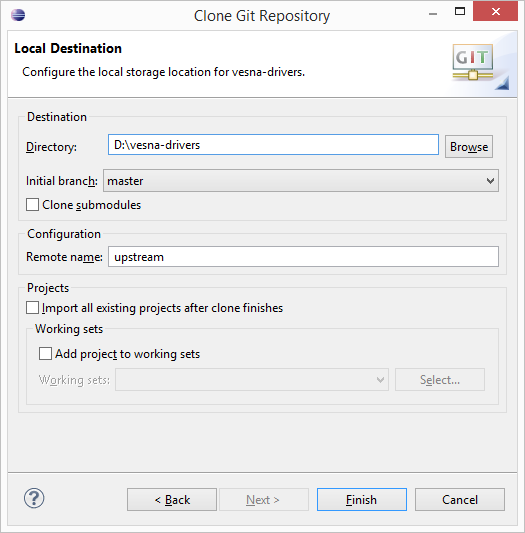
\includegraphics[scale=0.7]{./install-guide-win-images/eclipse-git-clone-repo-local-destination.png}
	\caption{Git repository local destination}
	\label{fig:eclipse-git-clone-repo-local-destination}
\end{figure}

\newpage

\subsection{Import project}

Now that the repository has been cloned you have to import it to Eclipse workspace.
Right-click on the \textit{"vesna-drivers"} repository in \textit{Git} perspective and select \textit{"Import Projects..."}. Select \textit{"Use the New project wizard"} and click \textit{Finish} (\autoref{fig:eclipse-git-import-project-select}).

\begin{figure}[H]
\centering
	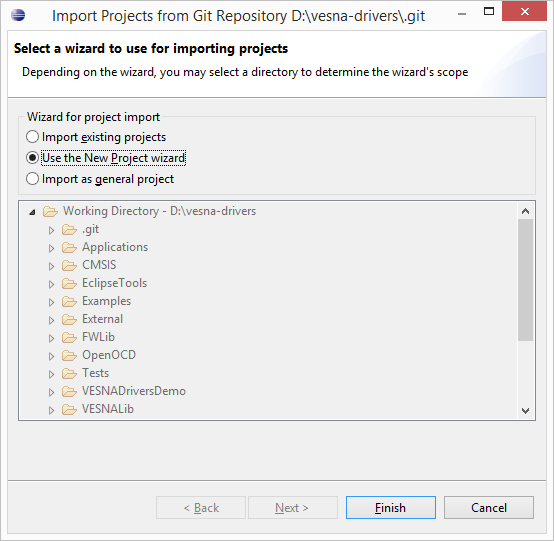
\includegraphics[scale=0.7]{./install-guide-win-images/eclipse-git-import-project-select.png}
	\caption{Project import wizard selection}
	\label{fig:eclipse-git-import-project-select}
\end{figure}

Now a new window opens. Select \textit{"C/C++ $\rightarrow$ Makefile project with Existing Code"} and click Next (\autoref{fig:eclipse-git-import-project-type}).

\begin{figure}[H]
\centering
	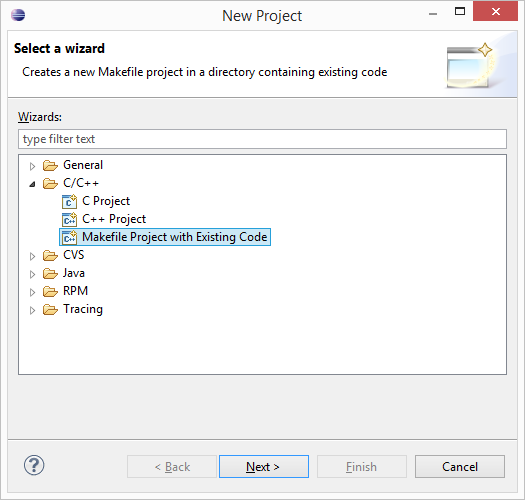
\includegraphics[scale=0.7]{./install-guide-win-images/eclipse-git-import-project-type.png}
	\caption{New project type selection }
	\label{fig:eclipse-git-import-project-type}
\end{figure}

Name the project \textit{"vesna-drivers"}, browse to the code location, select both C and C++ as the Language and select \textit{"Cross ARM GCC"} as the tool-chain (\autoref{fig:eclipse-git-import-project-existing-code}). The code is located in the directory you have selected as the Git repository location. Click \textit{Finish}.

\begin{figure}[H]
\centering
	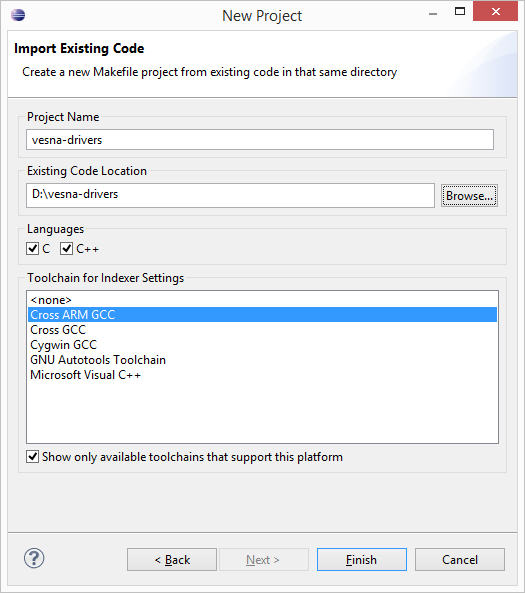
\includegraphics[scale=0.7]{./install-guide-win-images/eclipse-git-import-project-existing-code.png}
	\caption{Import existing code window}
	\label{fig:eclipse-git-import-project-existing-code}
\end{figure}

Switch to the \textit{"C/C++"} perspective. You can now see the project structure in \textit{"Project Explorer"}.

\newpage

\subsection{Configure the project}

In \textit{"Project Explorer"} right click on the top folder (vesna-drivers) and lef-click on \textit{"Properties"}. Go to \textit{C/C++ Build $\rightarrow$ Settings} and change the \textit{"Name"} field under \textit{"Toolchains"} to \textit{"Sourcery CodeBench Lite for ARM EABI (arm-none-eabi-gcc)"} (\autoref{fig:eclipse-project-properties-toolchain}).

\begin{figure}[H]
\centering
	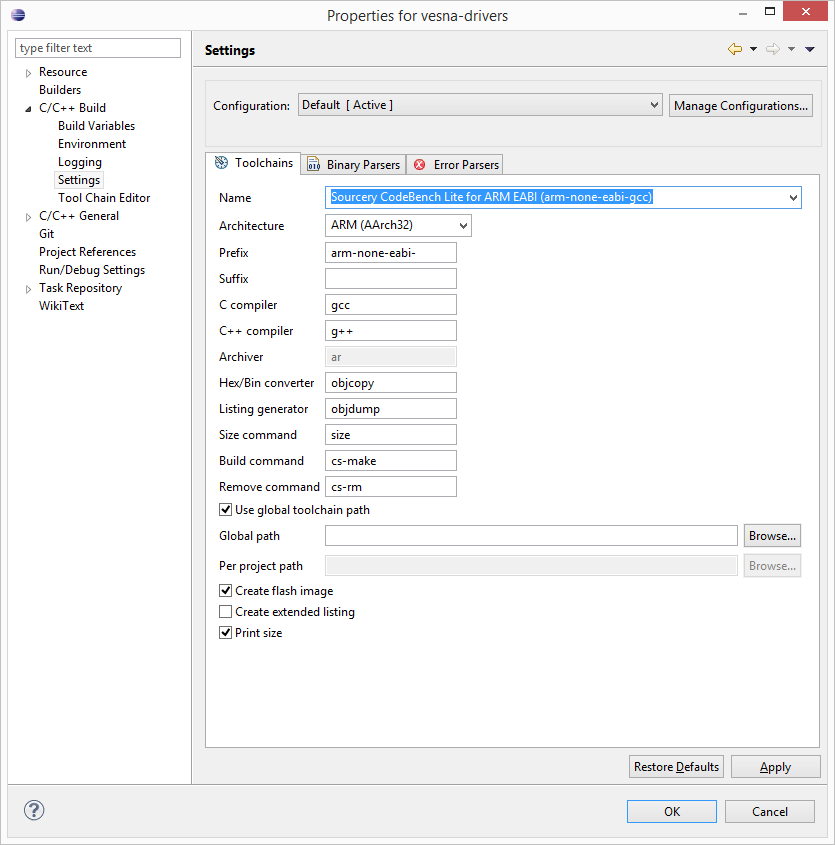
\includegraphics[width=0.9\linewidth]{./install-guide-win-images/eclipse-project-properties-toolchain.png}
	\caption{Project tool-chain settings}
	\label{fig:eclipse-project-properties-toolchain}
\end{figure}

Go to \textit{"C/C++ General"} and tick the  \textit{"Enable project specific settings"} box and select \textit{"Doxygen"} as the documentation tool (\autoref{fig:eclipse-project-properties-doxygen}).

\begin{figure}[H]
\centering
	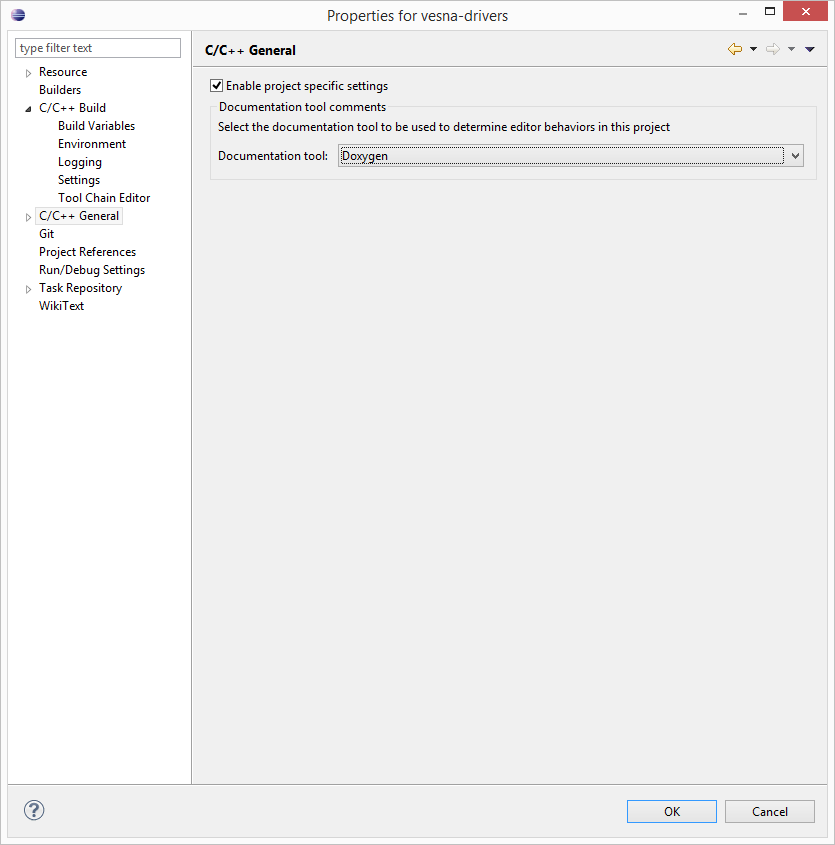
\includegraphics[width=0.9\linewidth]{./install-guide-win-images/eclipse-project-properties-doxygen.png}
	\caption{Documentation tool settings}
	\label{fig:eclipse-project-properties-doxygen}
\end{figure}

The basic project configuration is now complete. When working with Git the project configuration files are ignored and are not changed when you switch between different commits or branches. In general project import and configuration must be done only when the repository is cloned for the first time.

\newpage

\subsection{Compile the source}

Go to \textit{"C/C++"} perspective and in \textit{"Project Explorer"} open the \textit{"VESNADriversDemo"} folder. This is the demo project you will compile and upload to SNC (\autoref{fig:eclipse-project-demo-view}).

\begin{figure}[H]
\centering
	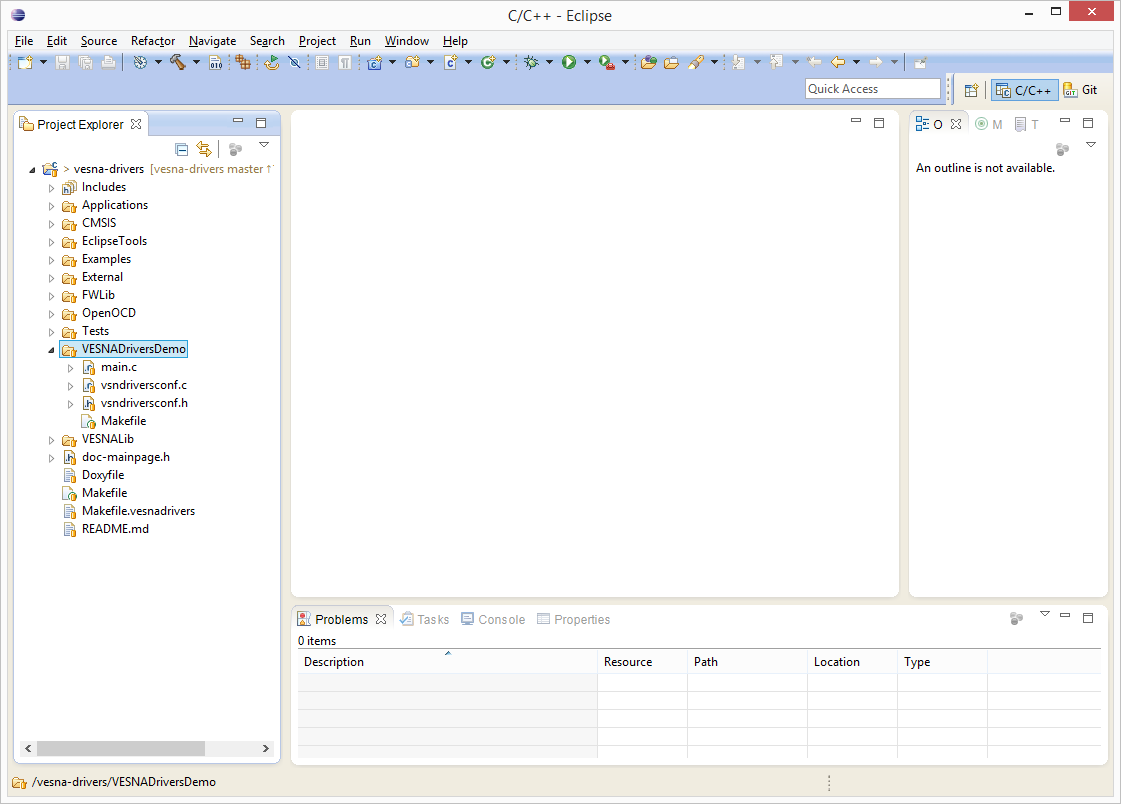
\includegraphics[width=0.9\linewidth]{./install-guide-win-images/eclipse-project-demo-view.png}
	\caption{C/C++ perspective demo project}
	\label{fig:eclipse-project-demo-view}
\end{figure}

The makefile system configures the code build process and all the needed files are build automatically. So that the build system knows what to build and how you need to pass it the correct make targets. The two basic targets are \textit{"all"} and \textit{"clean"} which build the project or remove all the build process files respectively.
Each project has at least two files \textit{"main.c"} and \textit{"Makefile"}. The file \textit{"main.c"} is the source of the main application code and the file \textit{"Makefile"} is part of the build system. To compile the code you have to append make targets to the \textit{"Makefile"}. You do this by right-clicking on the \textit{"Makefile"} and left-click on \textit{Make Targets $\rightarrow$ Create...} and fill in the \textit{"Target name"} first \textit{"all"} and then do the same thing for \textit{"clean"} (\autoref{fig:eclipse-create-make-target}).

\begin{figure}[H]
\centering
	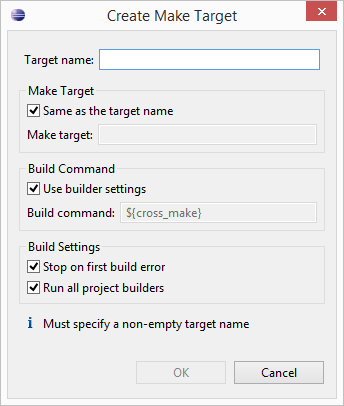
\includegraphics[scale=0.7]{./install-guide-win-images/eclipse-create-make-target.png}
	\caption{Create make target}
	\label{fig:eclipse-create-make-target}
\end{figure}

Find the \textit{"Make Target"} tab on the right side (\autoref{fig:eclipse-make-target-tab}). The folder structure is the same as in \textit{"Project Explorer"} but there are no files only make targets. To see the make targets you have just created open the \textit{"VESNADriversDemo"} folder. Double-click on the \textit{"all"} make target and the project will start building. You can follow the build process in the \textit{"Console"} tab at the bottom of the Eclipse window (\autoref{fig:eclipse-build-code}).

\begin{figure}[H]
\centering
	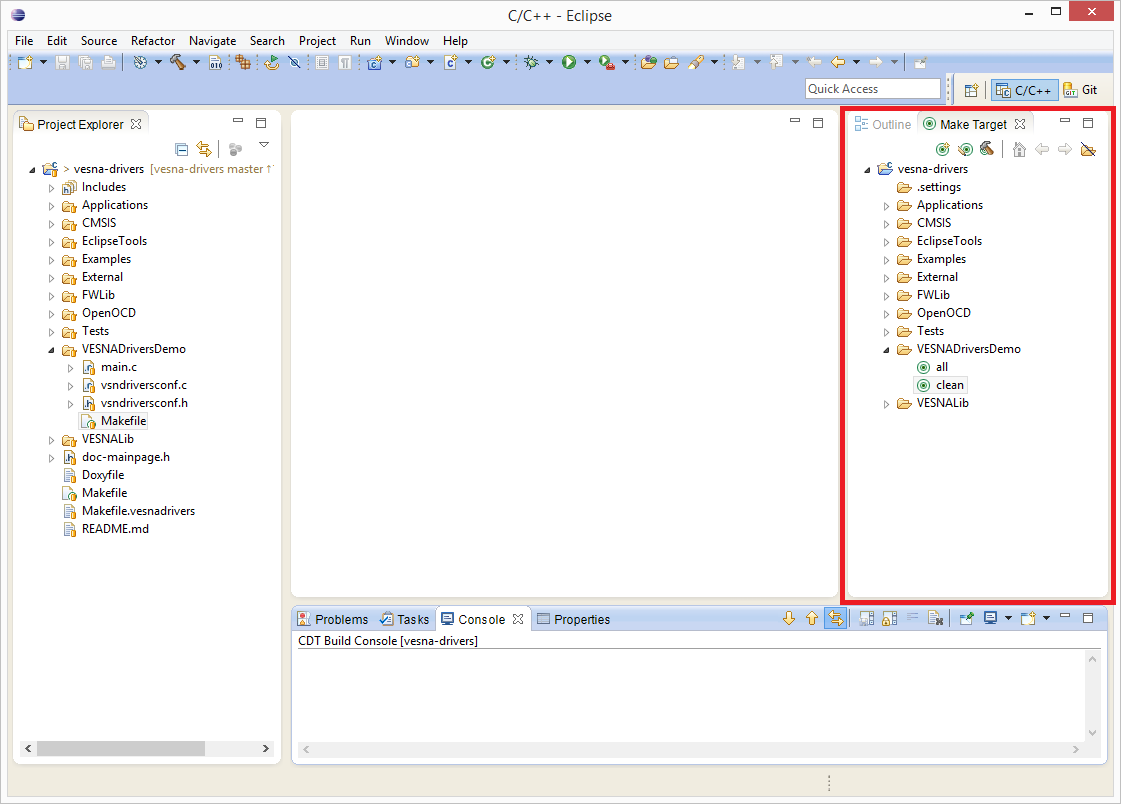
\includegraphics[width=0.9\linewidth]{./install-guide-win-images/eclipse-make-target-tab.png}
	\caption{"Make Target" tab (in red square)}
	\label{fig:eclipse-make-target-tab}
\end{figure}

\begin{figure}[H]
\centering
	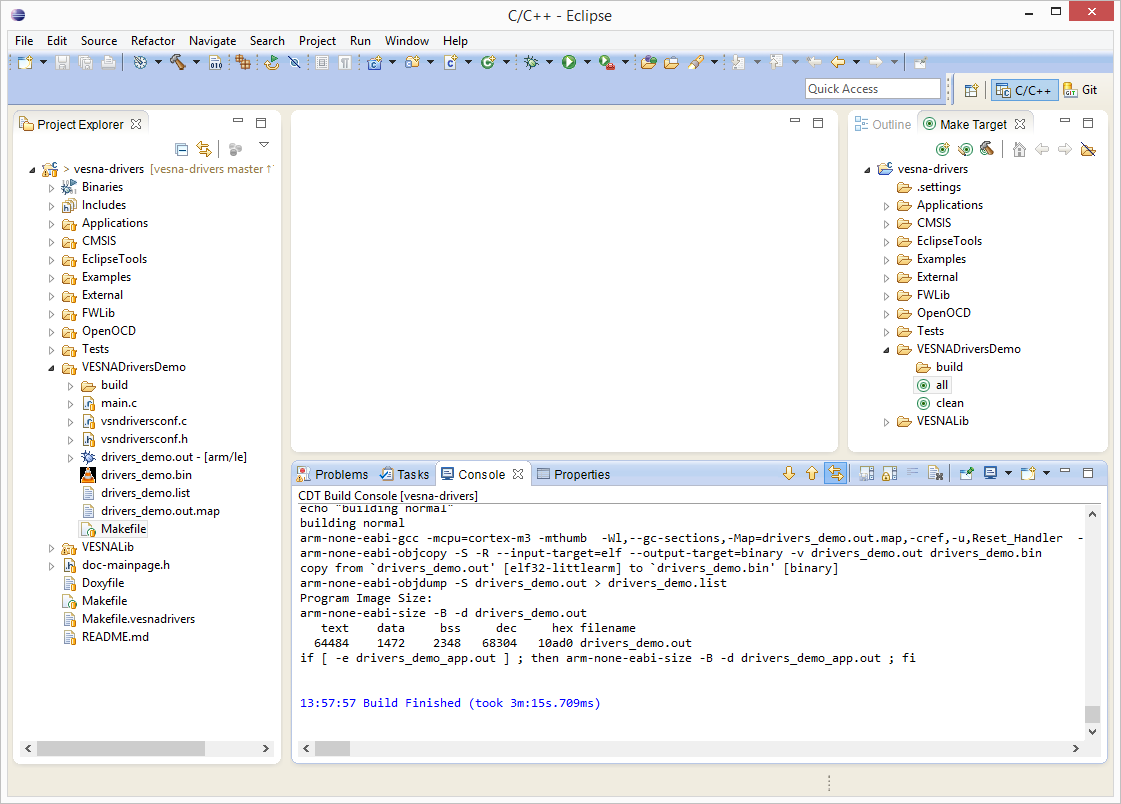
\includegraphics[width=0.9\linewidth]{./install-guide-win-images/eclipse-build-code.png}
	\caption{Building the code}
	\label{fig:eclipse-build-code}
\end{figure}

\newpage
\section{Upload the project and start debug}

Now connect the SNC board to the debugger and power supply. Click on the arrow in the \textit{"External Tools"} icon  and select \textit{"OpenOCD-STLinkV2 VESNA Drivers Debug"} (\autoref{fig:eclipse-external-tool-start}). This will start OpenOCD, connect STLink V2 debugger to OpenOCD and configure SNC for debugging.

\begin{figure}[H]
\centering
	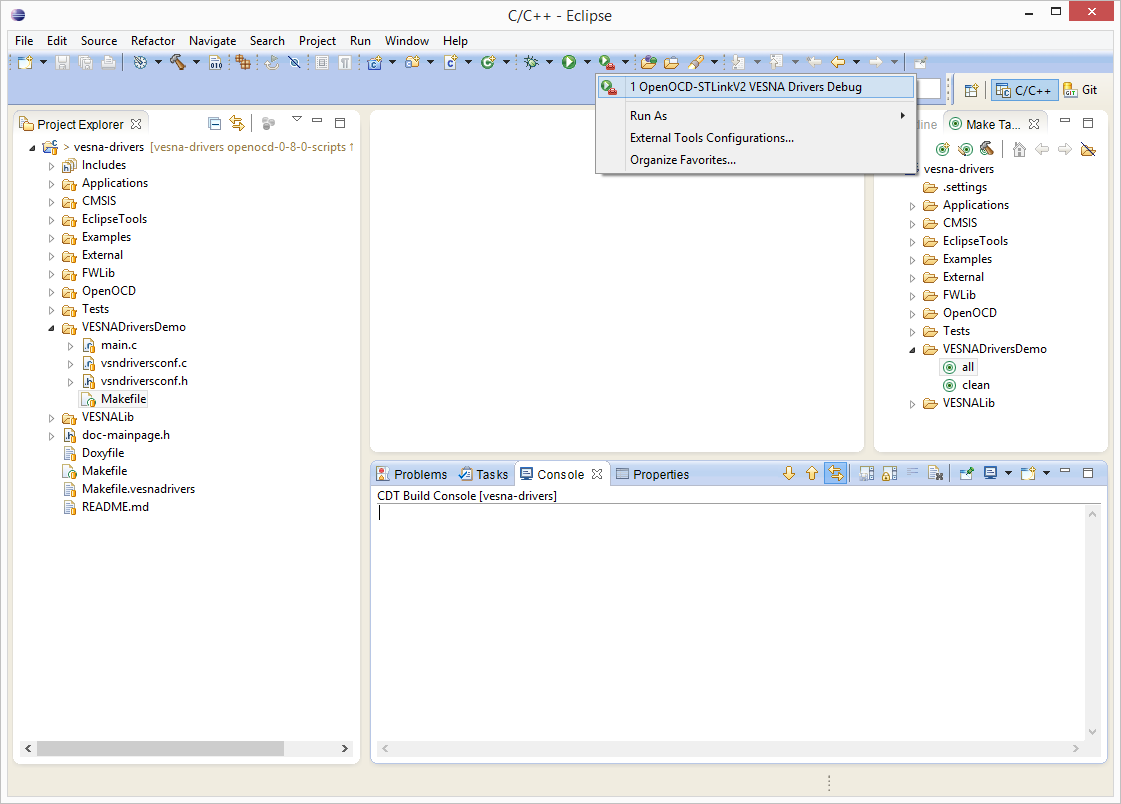
\includegraphics[width=0.9\linewidth]{./install-guide-win-images/eclipse-external-tool-start.png}
	\caption{External tool selection}
	\label{fig:eclipse-external-tool-start}
\end{figure}

If all is working you should see something like this in the \textit{"Console"} window on \autoref{fig:eclipse-external-tool-working}.

\begin{figure}[H]
\centering
	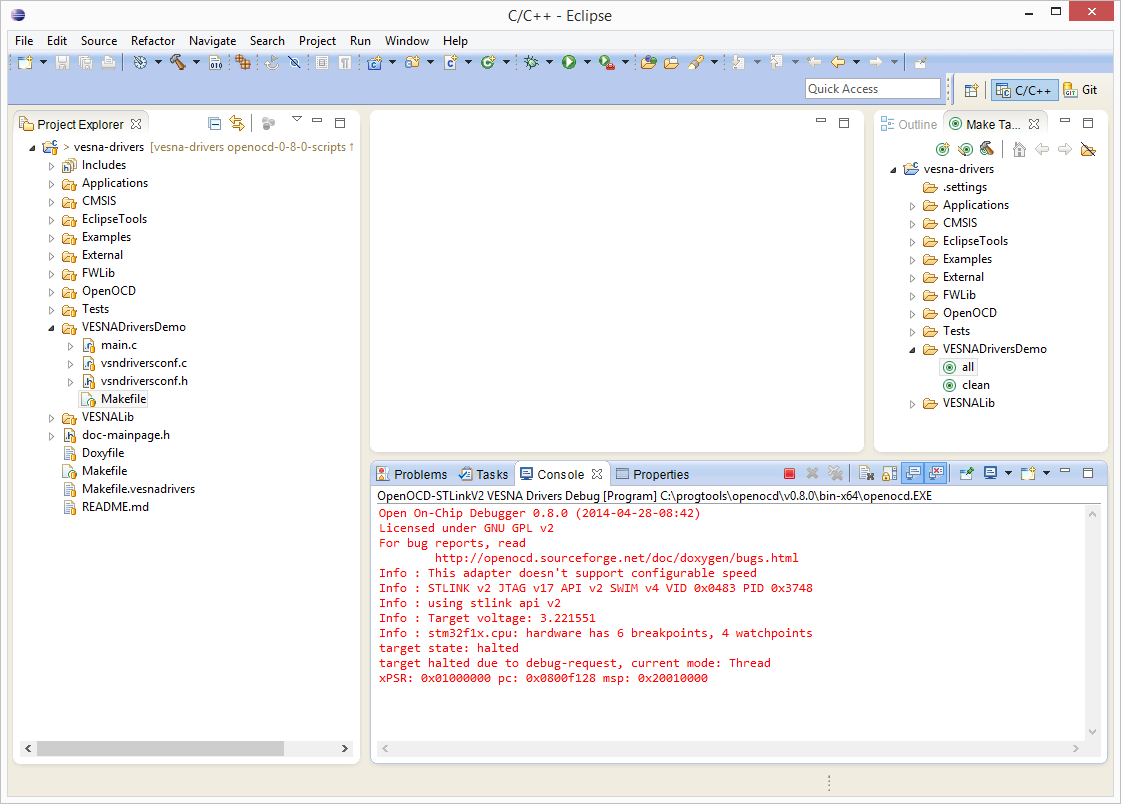
\includegraphics[width=0.9\linewidth]{./install-guide-win-images/eclipse-external-tool-working.png}
	\caption{External tool running}
	\label{fig:eclipse-external-tool-working}
\end{figure}

This means that the debugger hardware is found and it is connected to SNC. 
Now start the debugger by clicking on the arrow in \textit{"Debugger configuration"} icon  and click on the \textit{"VESNA Drivers Load and Debug"} (\autoref{fig:eclipse-debug-config-start}). This will upload the software to SBC and start the debugger. 

\begin{figure}[H]
\centering
	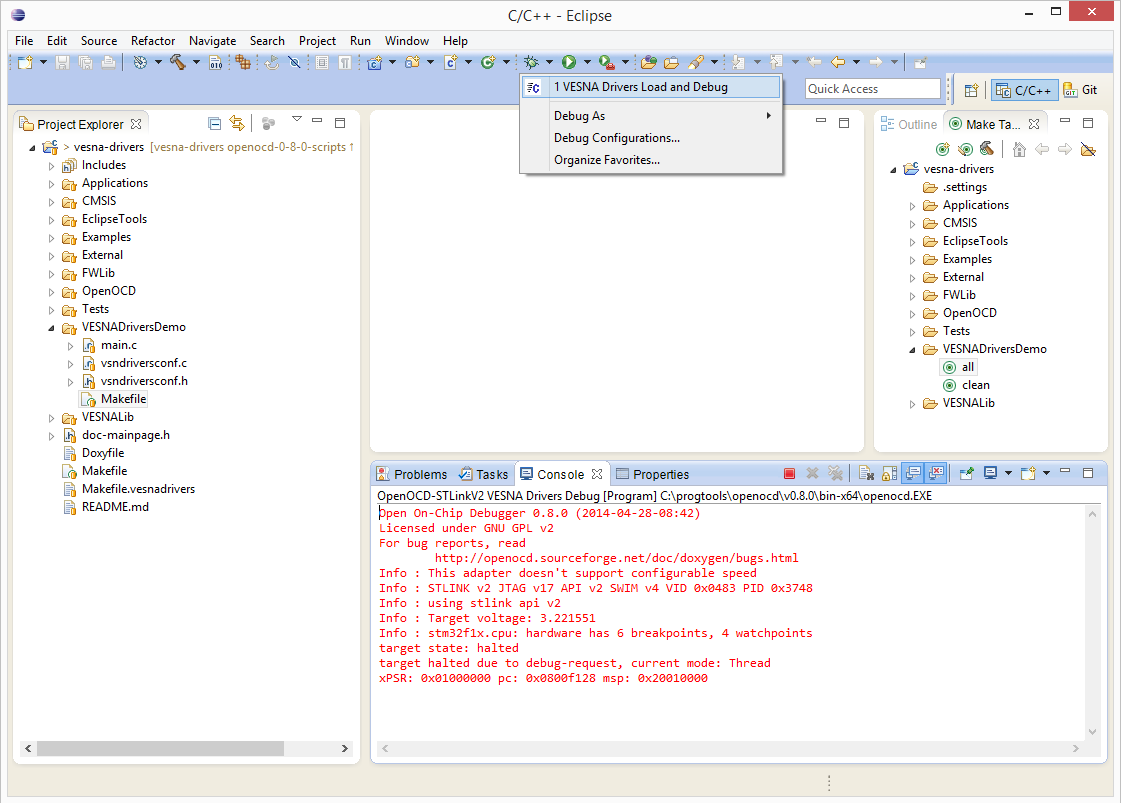
\includegraphics[width=0.9\linewidth]{./install-guide-win-images/eclipse-debug-config-start.png}
	\caption{Debugger configuration}
	\label{fig:eclipse-debug-config-start}
\end{figure}

You are prompted to switch the view to the \textit{"Debug"} perspective, click \textit{Yes} (\autoref{fig:eclipse-debug-config-switch-perspective}).

\begin{figure}[H]
\centering
	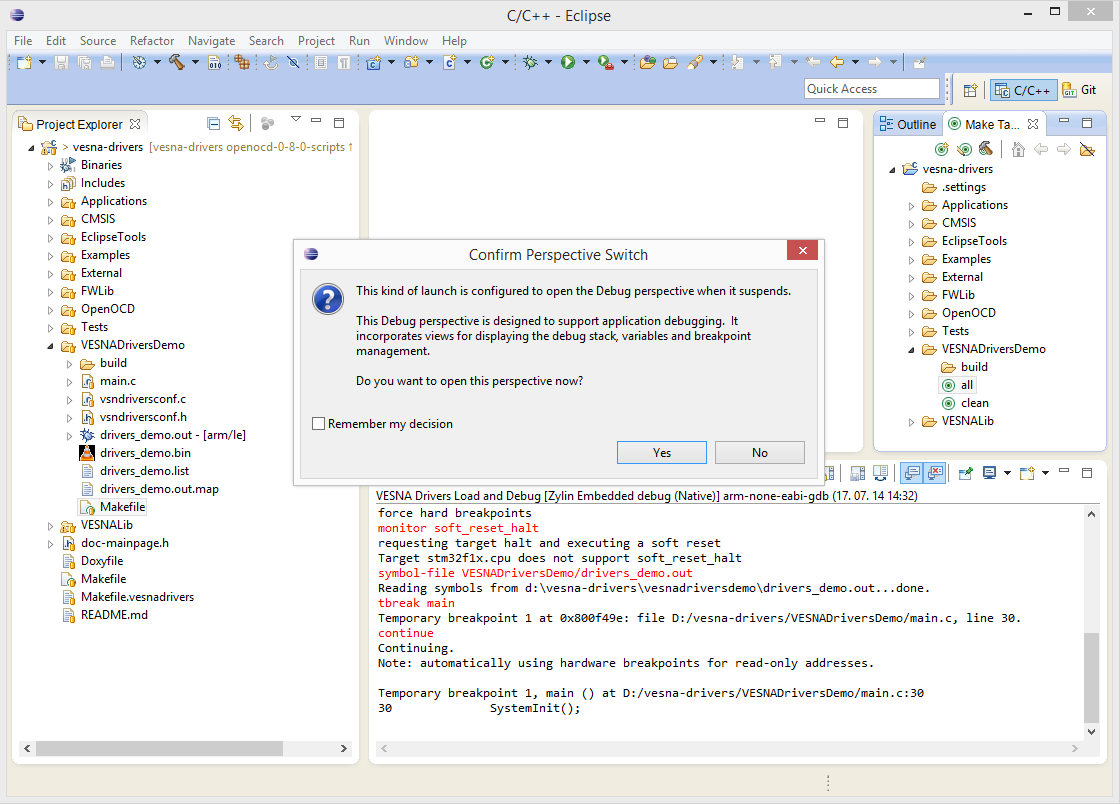
\includegraphics[width=0.9\linewidth]{./install-guide-win-images/eclipse-debug-config-switch-perspective.png}
	\caption{Prompt to switch to "Debug" perspective}
	\label{fig:eclipse-debug-config-switch-perspective}
\end{figure}

Now you should see something like \autoref{fig:eclipse-debug-perspective}. The program is automatically paused at the first line of main. The current position of the program in the code can bee seen in the code tab (green rectangle).
The pausing and running of the program can be controlled with the debug controls (yellow rectangle).
Variables can be inspected in the \textit{"Variables"} tab (red rectangle).
Running debug tools (OpenOCD and GDB) can be seen in the \textit{"Debug"} tab (blue frame). You can also see the current stack composition in the \textit{"Debug"} window if you look under the \textit{"Thread[1].."} line.

\begin{figure}[H]
\centering
	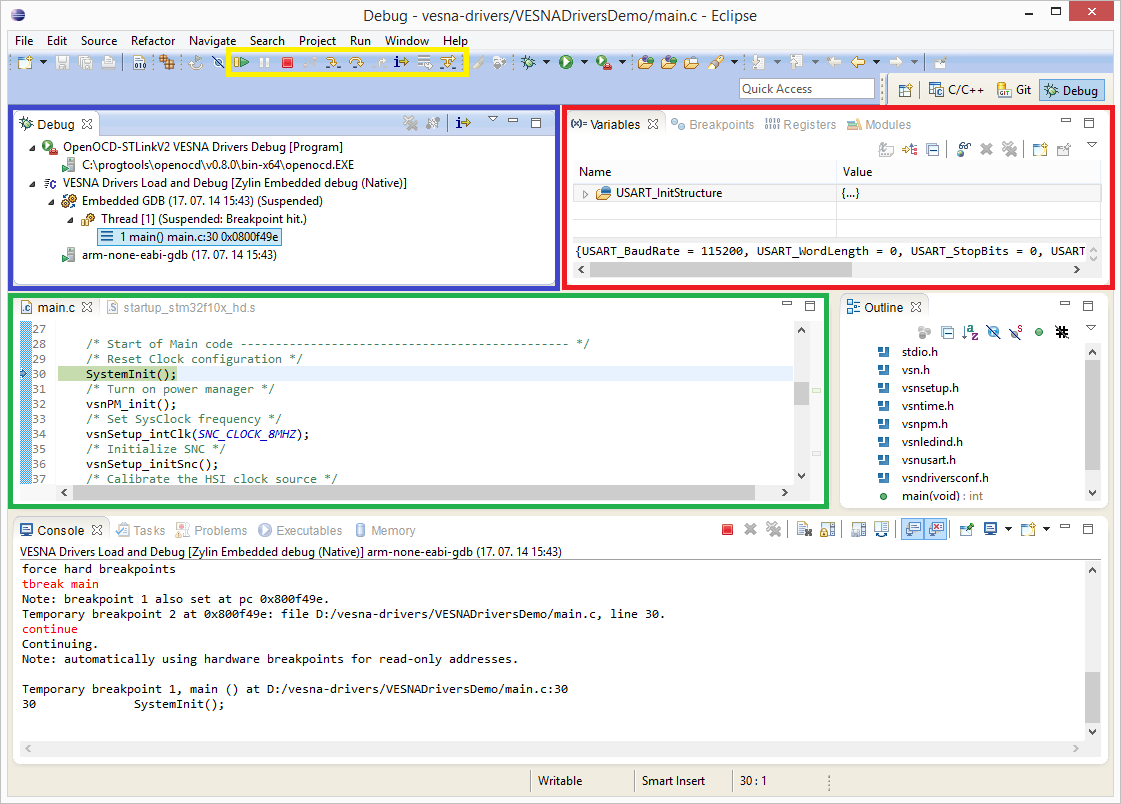
\includegraphics[width=0.9\linewidth]{./install-guide-win-images/eclipse-debug-perspective.png}
	\caption{Debug perspective, yellow frame: debug controls, blue frame: running debug tools and current stack position, red frame: local variables and green frame:  current position in code}
	\label{fig:eclipse-debug-perspective}
\end{figure}

\newpage

\begin{thebibliography}{9}
\bibitem{frtos}
	FreeRTOS.org STM32 demo using Eclipse, OpenOCD and GCC.
	\newline
	\url{http://www.stf12.org/developers/ODeV.html}
\bibitem{kt09}
	Kevin Townsend. Configuring Eclipse + OpenOCD + GCC to Debug NativeSample.
	\newline
	\url{http://msmicroframework.blogspot.com/2009/02/configuring-eclipse-openocd-gcc-to.html}
\bibitem{linfreak}
	Debugging STM32 Cortex-M3 microcontroller using Eclipse on Slackware.
	\newline
	\url{http://linuxfreak.pl/elektronika/debugging-stm32-cortex-m3-microcontroller-using-eclipse-on-slackware/}
\end{thebibliography}

\end{document}